\end{multicols}
\newpage
\begin{figure}[h]
\centering
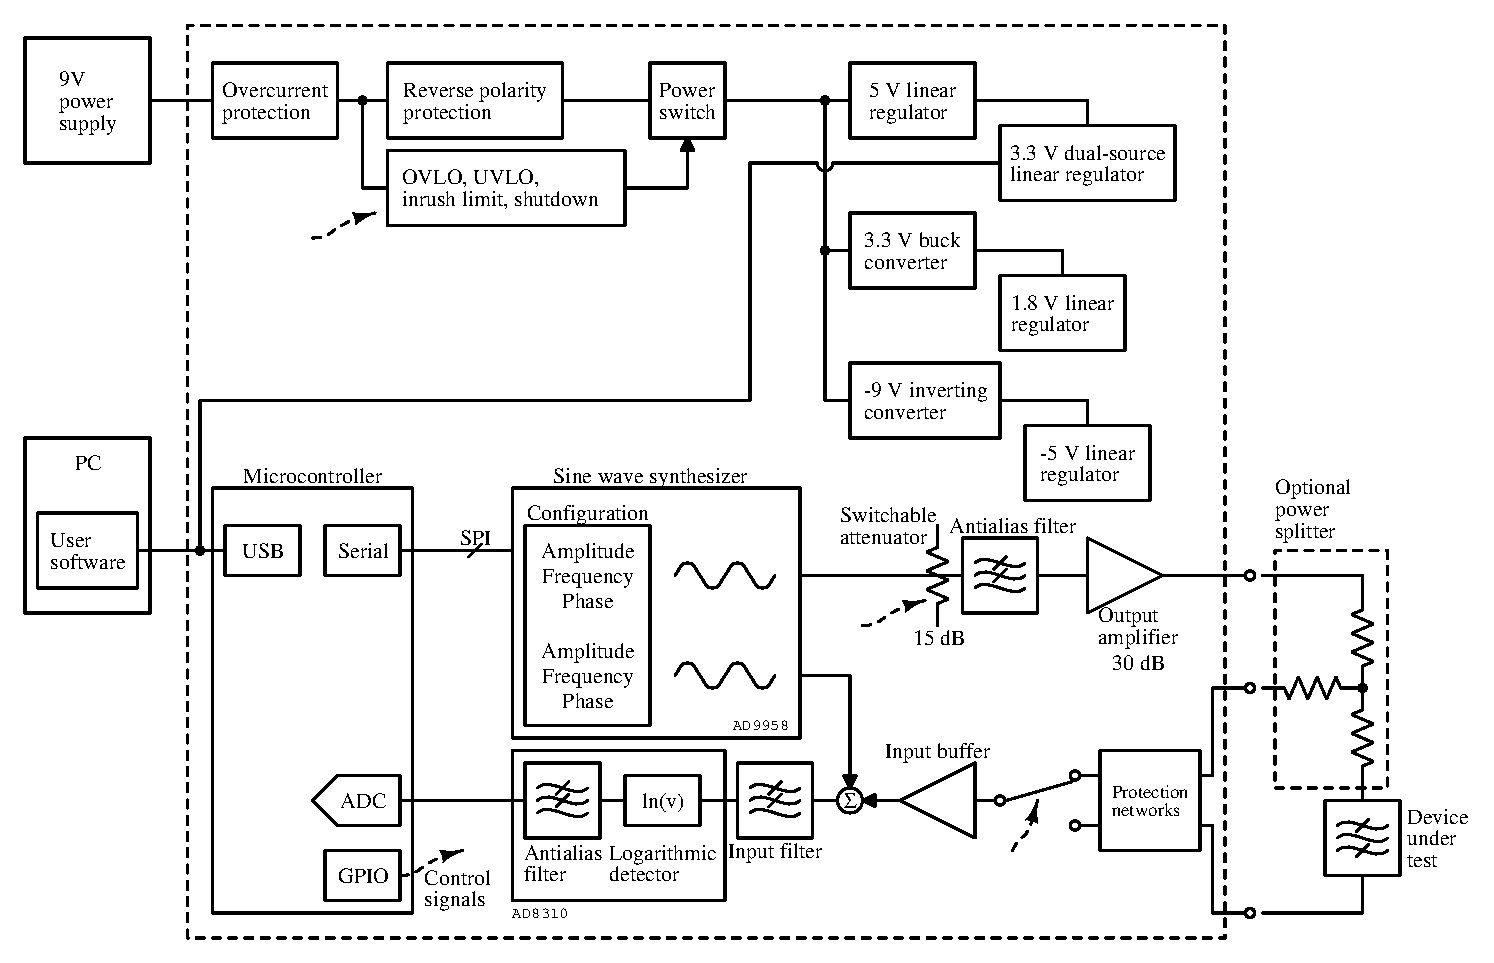
\includegraphics[width=6.5in]{blockdiagram}
\caption{Block diagram}
\label{fig:blockdiagram}
\end{figure}
\begin{multicols}{2}

\chapter{Theory of Operation}

This section contains a decription of the operation of the gain/phase analyzer.
Explanations range from simple and broad to very specific.
It is expected that the reader has an understanding of the basics of
gain/phase analysis itself, which is explained in the \hyperref[chap:intro]{Introduction
chapter}.

Also, it will be beneficial to look at the main system schematics when reading
through this section. Small pieces of the schematic are excerpted when helpful
in explaining their function, but are not always shown.

\section{Block Description}

The block diagram is shown in figure~\ref{fig:blockdiagram}. 
